\documentclass[a4paper, 11pt]{article}
\usepackage[portuguese]{babel}
\usepackage{style}

\title{\Huge Projeto BD 2024/2025\\
        \it \huge University Management System
}
\author{Base de Dados --- LEI 2024/2025}
\date{}

\begin{document}
\maketitle
\begin{center}
    \begin{tabularx}{0.8\textwidth}{Xcr}
    \bf Nome  & \bf Nº Estudante & \bf Contacto  \\\midrule
    Vasco Guilherme da Silva Alves & 2022228207 & 960399272\\
    Lucas Pinto Oliveira & 2023219472 & 969244925 \\ 
    João Tomás Gomes Forte Neto & 2023234004 & 967476669
    \end{tabularx}
\end{center}

\tableofcontents

% -----------------------------------------------------------------------------
% Abstract
% -----------------------------------------------------------------------------
\newpage
\section{Abstract}
O objetivo deste projeto é desenvolver competências que nos permitam realizar outros projetos envolvendo bases de dados. Para alcançar esse objetivo, pretendemos focar nas seguintes competências: 

\begin{itemize}
  \item Melhorar nossas habilidades de organização.
  \item Desenvolver modelos de dados eficientes e bem estruturados.
  \item Aprimorar nossa capacidade de criar modelos que atendam às necessidades dos projetos.
  \item Adquirir conhecimentos para instalar e configurar sistemas de gestão de bases de dados.
\end{itemize}

% -----------------------------------------------------------------------------
% Diagrama
% -----------------------------------------------------------------------------
\section{Diagrama}
\begin{figure}[h!]
    \centering
    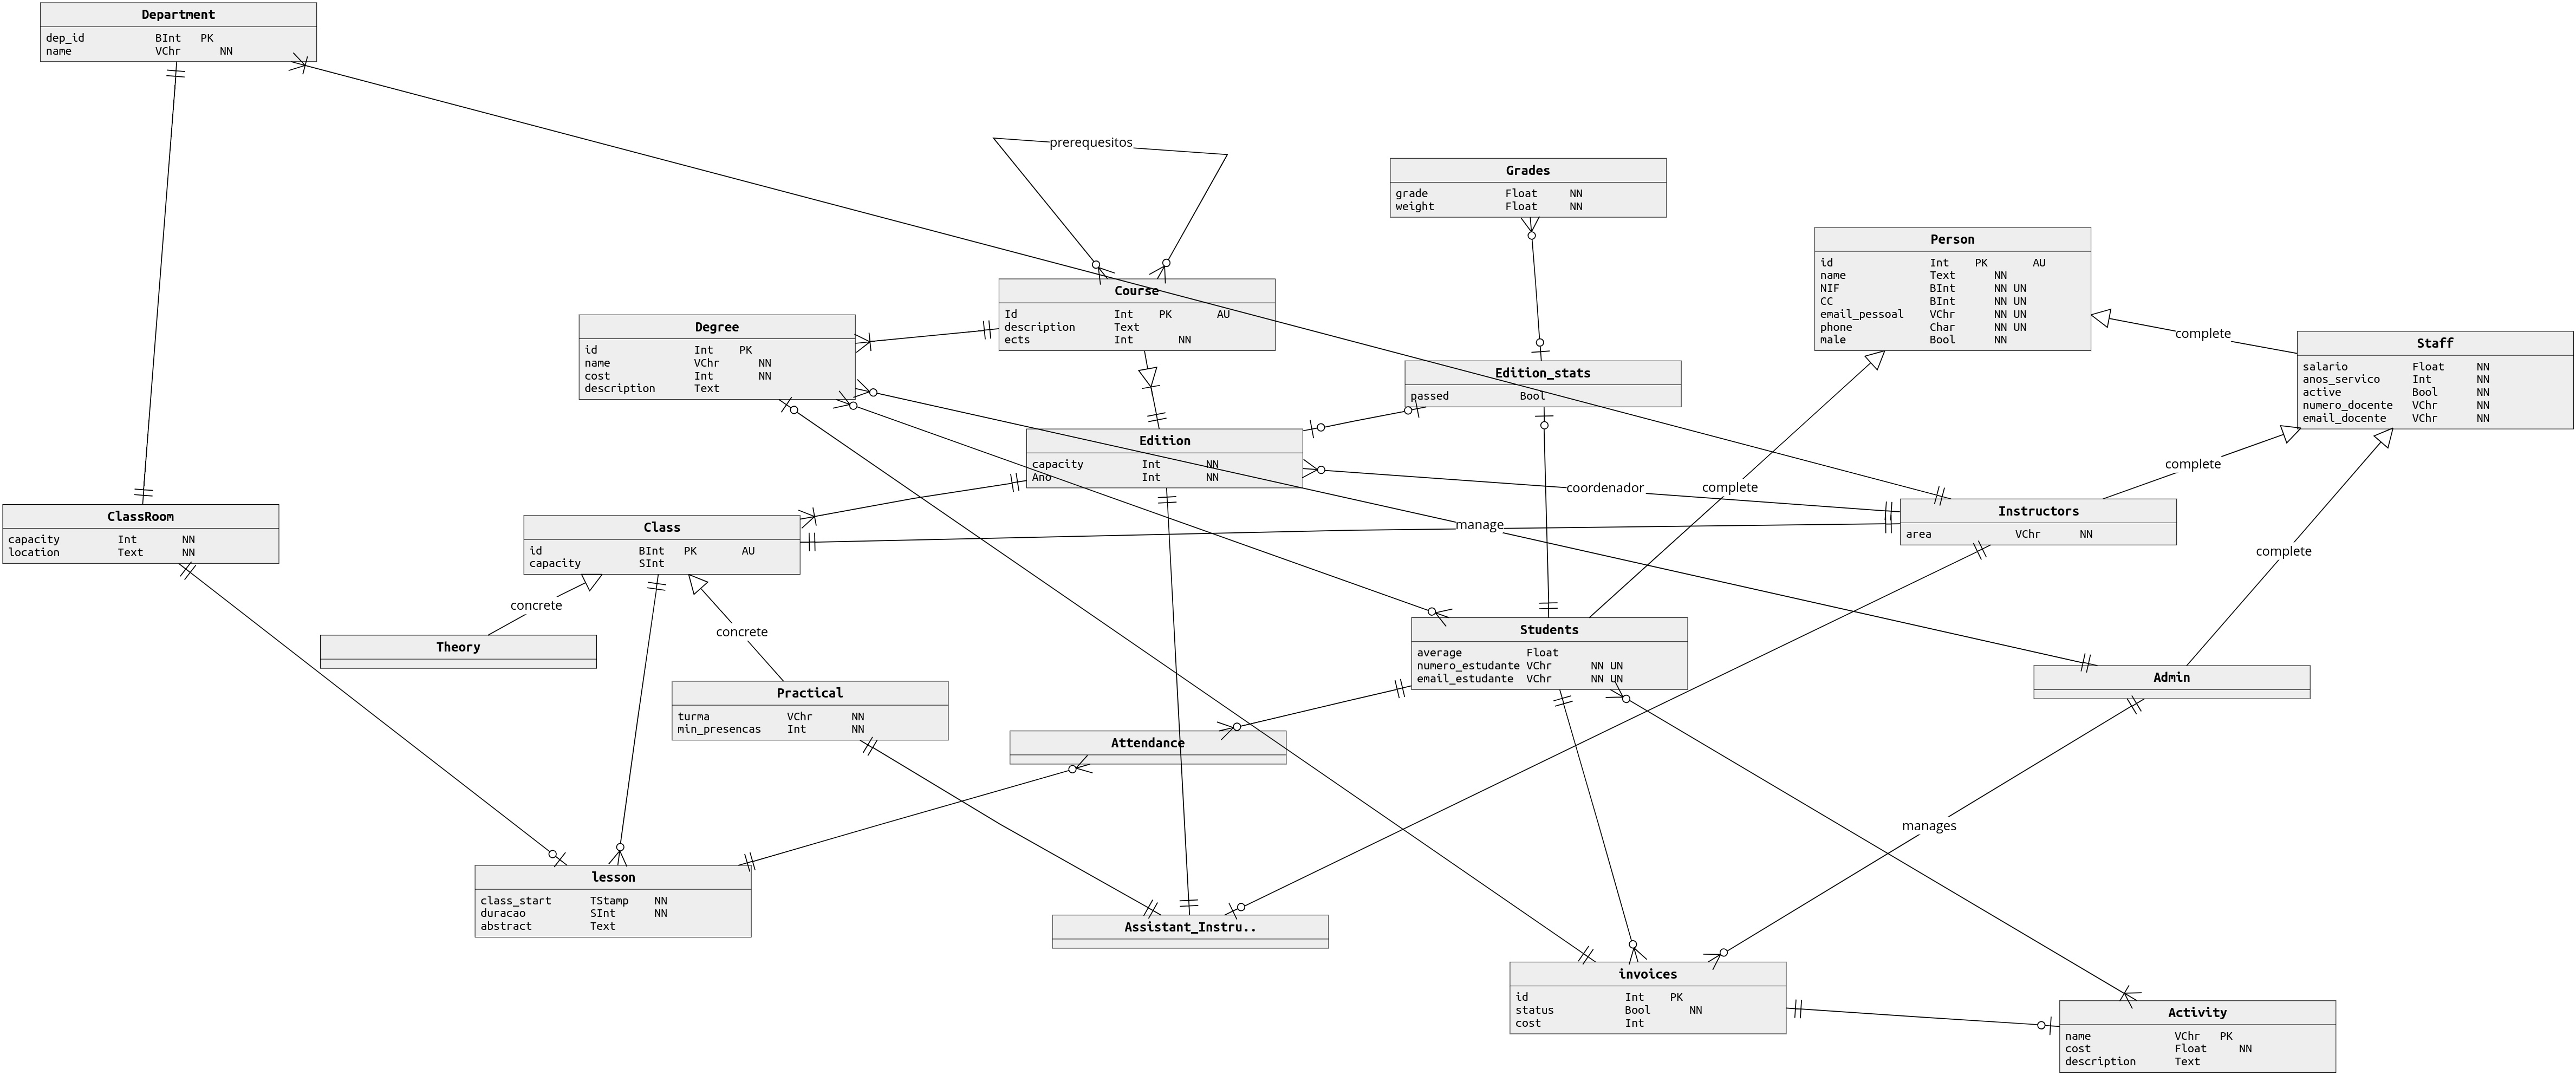
\includegraphics[width=0.95\textwidth]{mrbreast.png}
    \caption{Diagrama de Relacionamento de Entidades}
    \label{fig:tensa-bullet}
\end{figure}

% -----------------------------------------------------------------------------
% Transactions
% -----------------------------------------------------------------------------
\section{Transactions}
  Após uma discussão com o grupo todo achamos pertinente implementar o uso de transações nas seguintes operações: 

\begin{itemize}
  \item Inscrição de um aluno num curso (degree) por causa do débito que deve ser associado ao estudante;  
  \item Inscrição de um aluno numa cadeira (edition) por causa da capacidade máxima da cadeira; 
  \item Inscrição de um aluno numa atividade (activity) por causa do débito que deve ser associado ao estudante; 
\end{itemize}
  
% -----------------------------------------------------------------------------
% Potenciais Conflitos
% -----------------------------------------------------------------------------
\section{Potenciais Conflitos}
  Consideramos que podem ocorrer conflitos (principalmente de concorrência) nos seguintes casos:

\begin{itemize}
  \item Na criação de uma nova turma (class) por causa de sobreposição de aulas com outras turmas na mesma sala (classroom), ou mesmo capacidade da turma superior à sala;
  \item Ao inscrever um aluno numa turma, pode ocorrer sobreposição nas aulas das turmas que ele está inscrito; 
  \item A inscrição de um aluno numa cadeira (edition) por causa da capacidade máxima da cadeira;
\end{itemize}

\subsection{Soluções}

Para resolver o primeiro conflito devemos, ao criar uma turma, verificar antes se a sala de aulas já está ocupada; caso esteja, não poderemos criar uma turma com aquelas aulas. A mesma lógica se aplica à inscrição de um aluno numa turma; porém, esta última deve ser executada com o uso de transações para garantir que uma vaga não seja ocupada por um aluno que nem irá participar nessa turma.
O último possível conflito já é resolvido com as transações. Caso o aluno se tente inscrever numa cadeira e a cadeira já esteja cheia, não será possível se inscrever. Como esta operação é executada com transações, não será ocupada uma vaga numa cadeira em vão.

\section{Plano}

\begin{enumerate}
  \item \textbf{Quick Checkpoint 1}
    \begin{itemize}
      \item Instalação do DBMS: Cada membro da equipa fará a instalação nos seus PCs individuais.
      \item Manual de Instalação: Será criado pelo Lucas.
      \item Implementação da REST API: Será realizada pelo Vasco.
    \end{itemize}

  \item\textbf{Quick Checkpoint 2}
    \begin{itemize}
      \item Implementação do processo de autenticação: Será feito pelo João.
      \item Criação do Manual do Utilizador: Será realizado pelo Vasco.
    \end{itemize}

  \item \textbf{Final Delivery}
    \begin{itemize}
      \item Modelo de relação: Será criado pelo Lucas. 
      \item Revisão Final e Demonstração: Será realizada em conjunto por todo o grupo.
    \end{itemize}
\end{enumerate}


\section{Installation Manual}
% For example, Tristan Tate, pulled up a video, his favorite whiskey, Johnnie Walker. What do I do at duty-free? Fucking Johnnie Walker. That night, sipping the fucking Johnnie Walker in the war room by myself with him chilling. Why? I studied, bro.

\subsection{Clone Python API and Install Dependencies}
\texttt{git clone https://github.com/lvcxss/UniversityManagementSystem\\pip install -r requirements.txt}

\subsection{Installing PostgreSQL and creating the needed tables}
\subsubsection{Installing PostgreSQL}
\textbf{Step 1: Downloading PostgreSQL Installer}
Download the latest stable PostgreSQL Installer for Windows:www.enterprisedb.com/downloads/postgres-postgresql-downloads

\textbf{Step 2:Installing the PostgreSQL installer}
Depois de fazer download do PostgreSQL installer carregar duas vezes onde foi guardado o ficheiro, para abrir o PostgreSQL installer.
\textbf{Step 3: Navegar o installer}

% \newpage
\begin{minipage}{0.45\textwidth}
  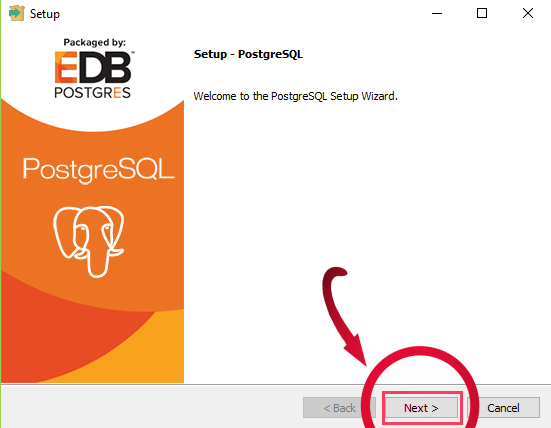
\includegraphics[width=\textwidth]{image.psd.png}
  1. Carregar no butão next
\end{minipage}\hfill
\begin{minipage}{0.45\textwidth}
  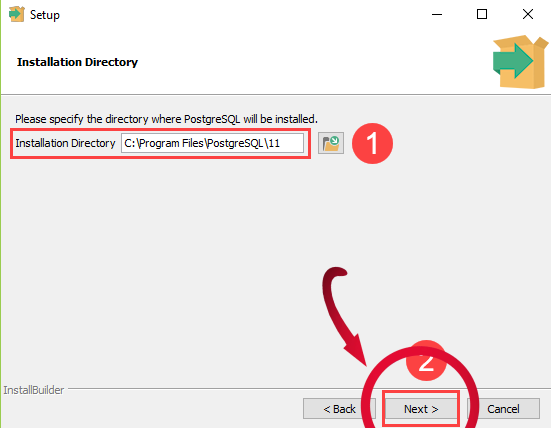
\includegraphics[width=\textwidth]{image.psd(1).png}
  2. Escolher uma pasta (default path é Program Files), e carregar no butão next
\end{minipage}

\begin{minipage}{0.45\textwidth}
  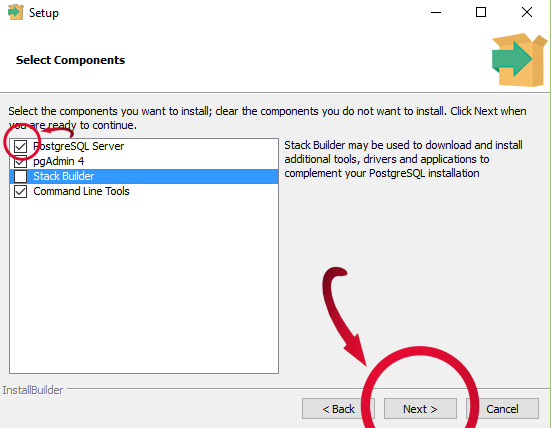
\includegraphics[width=\textwidth]{image.psd(2).png}
  3. Escolher os componentes para instalar (o unico componente necessario para utilizar a base de dados é PostgreSQL Server)
\end{minipage}\hfill
\begin{minipage}{0.45\textwidth}
  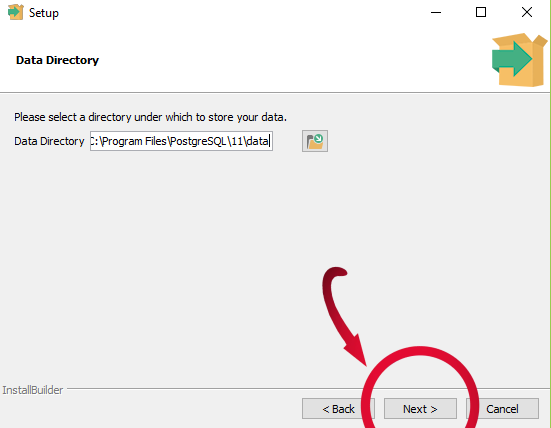
\includegraphics[width=\textwidth]{image.psd(3).png} 
  4. Escolher a pasta para o lugar onde a informação vai ser instalada e carregar next
\end{minipage}

\begin{minipage}{0.45\textwidth}
  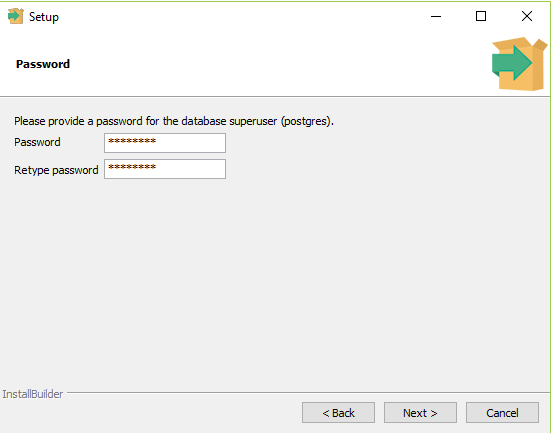
\includegraphics[width=\textwidth]{Screenshot-4109.png}  
  5. Escolher a password da database superuser(Importante não esquecer vai ser utilizado mais tarde) e carregar em next
\end{minipage}\hfill
\begin{minipage}{0.45\textwidth}
  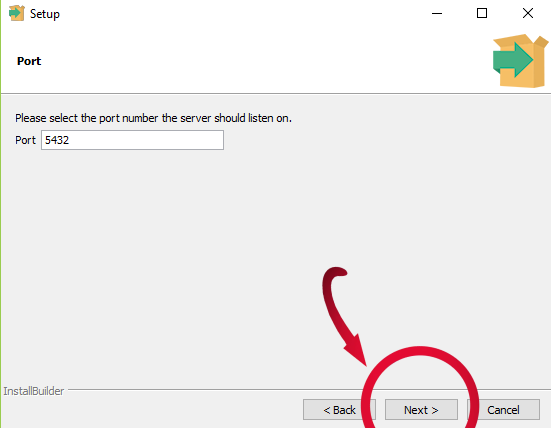
\includegraphics[width=\textwidth]{image.psd(4).png}
  6. Carregar em Next
\end{minipage}

\begin{minipage}{0.45\textwidth}
  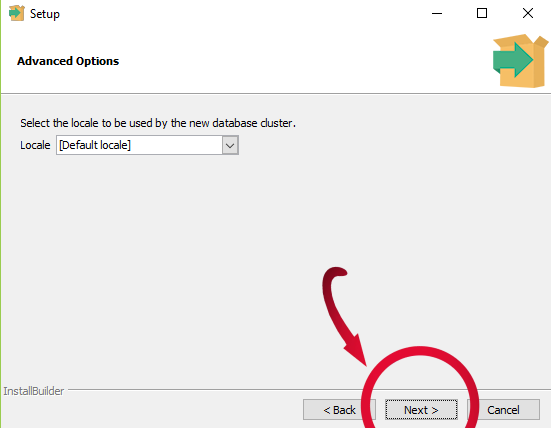
\includegraphics[width=\textwidth]{image.psd(5).png}
  7. Carregar em Next
\end{minipage}\hfill
\begin{minipage}{0.45\textwidth}
  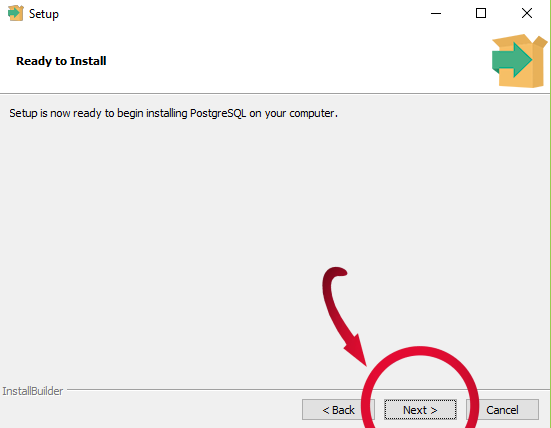
\includegraphics[width=\textwidth]{image.psd(6).png}
  8. Carregar em Next
\end{minipage}

\begin{minipage}{0.45\textwidth}
  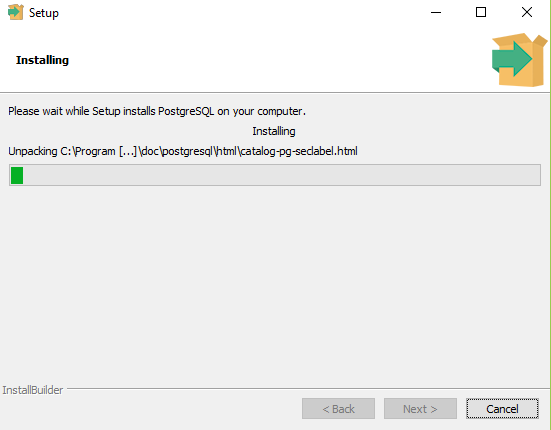
\includegraphics[width=\textwidth]{Screenshot-830.png}
  9. Esperar para instalar
\end{minipage}\hfill
\begin{minipage}{0.45\textwidth}
  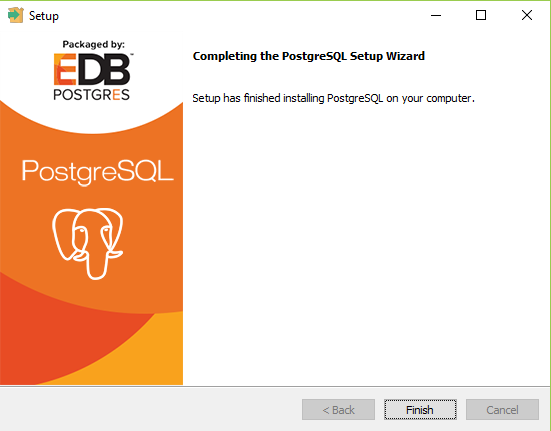
\includegraphics[width=\textwidth]{Screenshot-937.png}
  10. Carreger em Finish
\end{minipage}

\vspace{1em}

\subsection{Creating the needed features of the Database}
Now open SQL shell and enter with your PostgreSQL database and copy and paste this:

\texttt{pg\_dump -h localhost -p 5432 -U "insert\_your\_user\_name" -d "insert\_your\_database\_name" -f backup.sql }

This will create the needed triggers, functions and tables for running the code.

\newpage
\section{User Manual}

\newcommand\PUT{{\bfseries\color{Blue} PUT}}
\newcommand\POST{{\bfseries\color{BurntOrange} POST}}
\newcommand\GET{{\bfseries\color{Green} GET}}
\newcommand\DELETE{{\bfseries\color{Maroon} DELETE}}

\newcommand\requestpar[4]{
  \vspace{0.5em}
  \noindent
  {#1} \href{http://localhost:8080#2}{#2}\\{#3}
  \vspace{0.5em}
  \ifx\relax#4\relax\else
    \par\hfill\begin{minipage}{0.95\textwidth}
    {\texttt{#4}}
    \end{minipage} 
  \fi
  \par
  \vspace{1em}
}

\subsection{Overview dos Endpoints}
\requestpar{\PUT}{/dbproj/user}{Faz o login do utilizador, seja aluno, administrador ou docente, devolve um token correspondente.}{\{   "email": "behelita23@uc.pt", "password": "123" \}}
\requestpar{\POST}{/dbproj/register/student}{Regista um estudante novo, requer token de administrador.}{
\{
    "name":"slk",
    "email": "sk@skbu.com",
    "phone": "+999 133 156 563",
    "cc" : 122111,
    "nif" : 218128,
    "password" : "123", 
    "gender" : "M",
    "email\_institucional": "cmi@uc.pt", 
    "numero\_estudante" : "uc232442", 
    "average" : 17
\}
}
\requestpar{\POST}{/dbproj/register/staff}{Regista um administrador novo, requer token de administrador.}{
\{
  "name":"behelitta",
  "email": "behelita@gmail.com",
  "phone": "+351 123 666 123",
  "cc" : 1234566,
  "nif" : 98724198421,
  "password" : "123",
  "gender" : "M",
  "email\_institucional" : "behelita23@uc.pt",
  "numero\_docente" : "uc200032",
  "salario" : 7128,
  "anos\_servico" : 4,
  "active" : true
\}}
\requestpar{\POST}{/dbproj/register/instructor}{Regista um docente novo, requer token de administrador.}{
\{
    "name":"cleverson",
    "email": "2@skbi.com",
    "phone": "+351 111 223 123",
    "cc" : 9251,
    "nif" : 522,
    "password" : "123", 
    "gender" : "M",
    "email\_institucional" : "cuh@uc.pt",
    "numero\_docente" : "uc1111",
    "salario" : 9994, 
    "anos\_servico" : 4, 
    "active" : true,
    "area" : "comp sci"
\}
}
\requestpar{\POST}{/dbproj/enroll\_degree/<degree\_id>}{Permite registar um utilizador num curso.}{
\{ "student\_id":9 \}}
\requestpar{\POST}{/dbproj/enroll\_activity/<activity\_id>}{Permite ao utilizador que fez login registar numa atividade.}{}
\requestpar{\POST}{/dbproj/enroll\_course\_edition/<course\_edition\_id>}{Permite ao utilizador que fez login registar em turmas.}{\{ "classes": [1, 2]
\}}
\requestpar{\POST}{/dbproj/submit\_grades/<course\_edition\_id>}{Permite ao regente da edição da cadeira submeter notas para os alunos.}{
  \{
    "period\_id": 1,
    "grades": [[23, 1]]
\}}
\requestpar{\GET}{/dbproj/student\_details/<student\_id>}{Devolve informação sobre as cadeiras em que o aluno está inscrito.}{}
\requestpar{\GET}{/dbproj/degree\_details/<degree\_id>}{Devolve informação sobre o curso e as respectivas edições.}{}
\requestpar{\GET}{/dbproj/top3}{Devolve os 3 melhores alunos do ano lectivo atual organizados por curso e atividades.}{}

\requestpar{\GET}{/dbproj/top\_by\_district/}{Devolve os melhores alunos de cada districto.}{}
\requestpar{\GET}{/dbproj/report}{Devolve as edições com o maior número de aprovações por mês.}{}
\requestpar{\DELETE}{/dbproj/delete\_details/<student\_id>}{Apaga o utilizador.}{}

\end{document}
